\section{总体分析}

\subsection{数据处理与边界闭合}

附件一给出的烘房温度与环境水分量具有明确时间顺序。为保留观测折点而不引入过冲，观测区间内采用分段线性插值；问题三、四超过4 h后，将3--4 h（含端点）的观测均值作为平台值，即
\[
T_{\mathrm{air}}=49.998934\ ^\circ\mathrm C,\qquad
C_{\mathrm{eq}}=0.0499875.
\]
其中$C_{\mathrm{eq}}$表示药材表面一侧的等效平衡含水率。空气水分量与药材干基含水率的参照质量不同，题目又未给出解吸等温线，故主情景取$C_{\mathrm{eq}}=Y$作为边界闭合。第\ref{sec:sensitivity}节除考察基准附近扰动外，还将$C_{\mathrm{eq}}=\beta Y$扩展到$\beta=0.5$--$2.8$，检验长期平衡含水率接近停机阈值时的终点变化。

附件二的半径观测在0--72 h内采用分段线性插值，问题四在51.0920 h即达到阈值，故无需外推半径。保形三次插值仅作为敏感性对照；它未在留出检验中表现出一致优势，因此不替换主方案\cite{fritsch1980}。

\subsection{尺度分析与模型选择}

设有效体积热容$b=\hat\rho c_p$、热扩散率$\alpha=k/b$，以初始半径$R_0$为特征长度，定义
\[
\tau_T=\frac{R_0^2}{\alpha},\qquad
\tau_C=\frac{R_0^2}{D},\qquad
Bi_T=\frac{hR_0}{k},\qquad
Bi_C=\frac{h_mR_0}{D}.
\]
三套物性的初始热扩散时间约为39.48、46.03和84.93 min，而水分扩散时间约为22.50、19.69和106.11 h；相应$Bi_T$和$Bi_C$均不满足小Bi数集总近似条件。因此，温度和含水率都保留径向分布。图\ref{fig:inputs-scales}同时展示外部驱动与材料尺度：烘房环境在数小时内接近平台，但水分扩散和收缩延续更久，不能把环境稳定时刻当作药材干燥终点。

\begin{figure}[htbp]
  \centering
  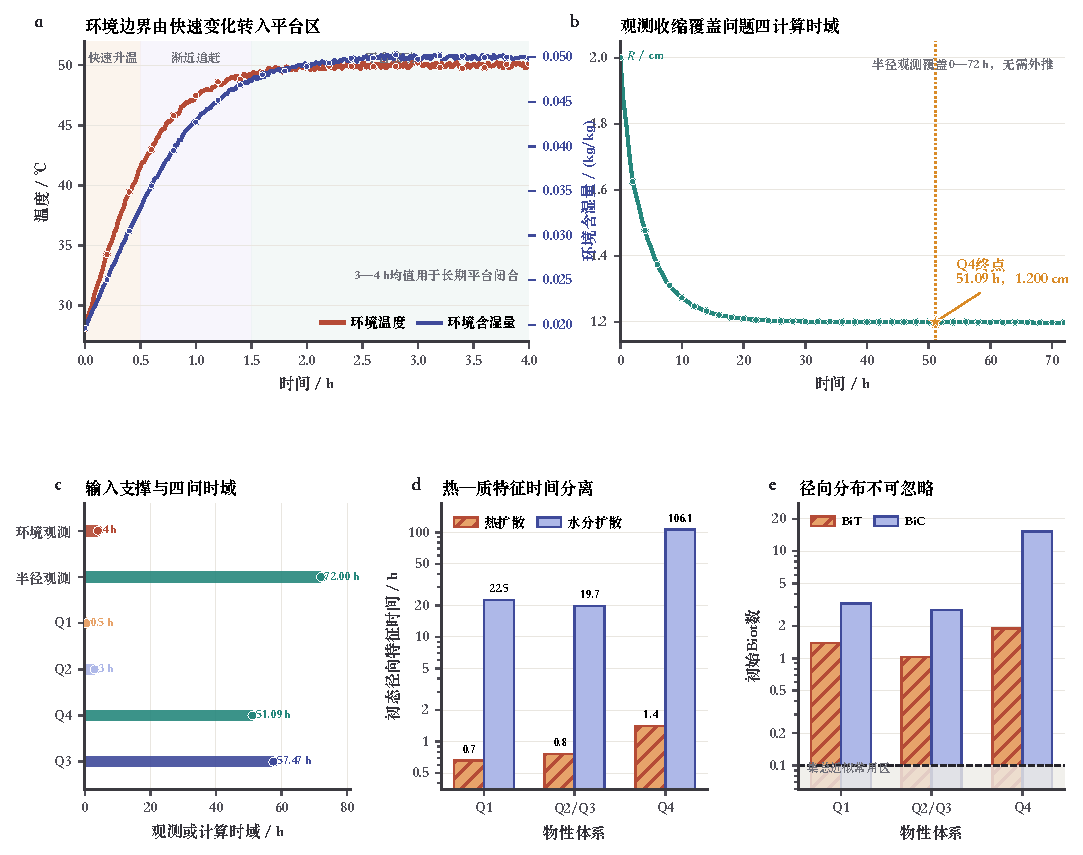
\includegraphics[width=\textwidth]{figures/fig01_inputs_scales.pdf}
  \caption{环境驱动与特征尺度}
  \label{fig:inputs-scales}
\end{figure}

图\ref{fig:inputs-scales}(c)把观测支持与计算时域放在同一时间轴上：环境仅观测至4 h，故问题三、四必须显式声明长期平台闭合；半径观测覆盖72 h，超过问题四的51.0920 h终点，不需要几何外推。图\ref{fig:inputs-scales}(d)(e)又表明三套物性的水分时间尺度均显著长于热时间尺度，且初始$Bi_T$、$Bi_C$均远高于集总近似常用界限0.1。这两条证据共同支持“保留径向分布、分别处理观测内插与长期延拓”的模型选择。

\subsection{四问的递进关系}

问题一中热学物性为常数，扩散率只依赖含水率，温度场和水分场可分别求解；问题二、三中$T$影响$D$，$C$又影响$D$、$b$和$k$，形成物性系数介导的双向反馈；问题三关注最后一个未达标位置，事件函数取全域最大含水率；问题四中半径随时间改变，需要在材料参考坐标中写出守恒方程。四问的核心依次是早期边界层、变物性反馈、阈值事件定位和移动域守恒。

表\ref{tab:problem-progression}列出四问之间“继承什么、增加什么”的关系。除问题三续接问题二的同一轨迹外，其余各问均从题给原始初态重算，避免把不同物性模型的末态错误串联。

\begin{table}[htbp]
  \caption{四问建模递进}
  \label{tab:problem-progression}
  \centering
  \begin{tabularx}{0.98\textwidth}{cXXX}
    \toprule
    问题 & 模型新增因素 & 初态与时间范围 & 核心输出 \\
    \midrule
    一 & 固定域解耦热传导与水分扩散 & 原始初态，0--30 min & 题定时空温湿场 \\
    二 & 状态相关物性与双向热湿反馈 & 原始初态，0--3 h & 前三小时耦合响应 \\
    三 & 全域最大值事件与严格判停 & 续接问题二，直至达标 & 临界时间及全程剖面 \\
    四 & 实测径向收缩与材料坐标 & 原始初态，直至达标 & 移动域终点及因素分解 \\
    \bottomrule
  \end{tabularx}
\end{table}
